\chapter{Software for experiment control and analysis}\label{chap:software}

\lettrine[lines=3]{S}{oftware underlies a huge part} of physicists' work, whether experimental or theoretical. On the experimental side, increasingly complex and precise experiments in atomic physics require increasingly sophisticated control of the lasers, magnetic coils, frequency synthesisers, cameras, etc.~that interact with the quantum systems being studied. Use of these devices necessitates some kind of interface between the experimentalist and each device, and whilst interfaces of the past were more likely to be knobs and dials on the front of the device, they are increasingly taking the form of software. Software is needed to convert from a smooth ramp of voltages designed to ramp up a magnetic field slowly into a finite list of voltages and times that a device can output with precise timing to make it happen. Software is needed to transmit this data to the device in question, using a communications protocol and data format compatible with the device. Software is required to extract the images from cameras and voltage time series from acquisition devices and store them in computer memory or on disk. And finally, software is required to compute meaningful results from this raw data.

A significant fraction of my PhD was spent developing, maintaining and improving the laboratory control system software suite that has emerged from the Quantum Fluids group at Monash: the \emph{labscript suite}. Originally envisioned as a Python~\cite{python_software_foundation_python_2018} library for generating instructions for programmable hardware via a LabVIEW~\cite{national_instruments_laboratory_2018} graphical interface, the software suite grew to encompass most aspects of day-to-day control and analysis in our labs. At present it comprises several separate programs/libraries---depending on how one chooses to draw the borders between them---that control every aspect of a cold atom physics experiment, from setting parameters to analysing results. An overview of the process is shown in Figure~\ref{fig:labscript_flowchart}.

The types of experiments the labscript suite addresses are `shot-based'---ones in which precise timing is required over hardware during some interval while a sequence of instructions is executed (a `shot'), after which the hardware is idle until the next shot. Many repetitions of similar shots are often performed to build up measurement statistics or investigate the response of a system to a change in  one or more parameters. This general method of hardware control and data acquisition is common to many experiments in cold quantum gases and trapped ions~\cite{robins_atom_2013-1, cronin_optics_2009-1}, quantum computation~\cite{negretti_quantum_2011-1, ladd_quantum_2010-1}, and quantum simulation~\cite{bloch_quantum_2012-1, blatt_quantum_2012-1}.

In this chapter, I'll first give a quick overview of each program and what it does. Then I'll outline the design and development approaches we undertook with the labscript suite and comment on the effects these choices have had on the course of the project in subsequent years. Then I'll summarise developments since the publication of our paper on the software, \emph{A scripted control system for autonomous hardware-timed experiments}~\cite{starkey_scripted_2013}, which is reproduced at the end of this chapter. I will also discuss our development roadmap. Further details on the role of each program in the suite and the design underlying it are available in the paper, and a more thorough presentation of the software, its design principles, comparisons with other laboratory control software, and recent and future developments are available in Philip Starkey's thesis~\cite{starkey_thesis_2018}.

\begin{figure}
\begin{center}
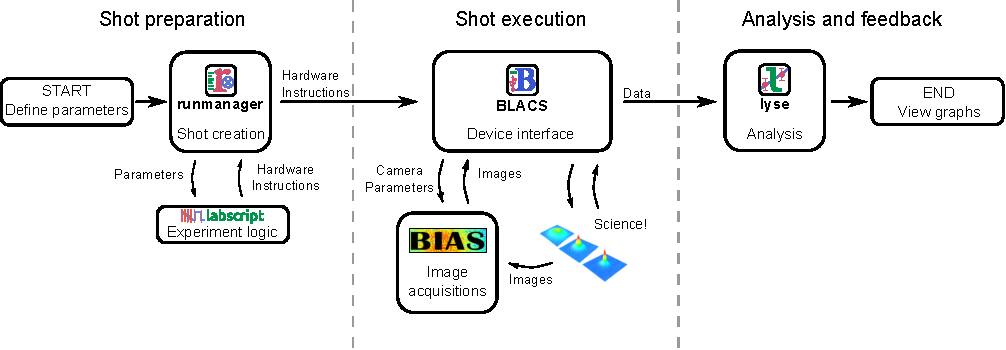
\includegraphics[width=\textwidth]{figures/software/flow_chart_simple-eps-converted-to.pdf}
\caption{The labscript suite comprises a number of libraries and programs allowing one to perform precisely timed experiments, each realisation of which we call a `shot', using commodity hardware such as devices from SpinCore, NovaTech, National Instruments and others. Experiment logic is described by the user in the form Python code using the \texttt{labscript} Python module, which produces from the user's code a set of low-level instructions appropriate for being programmed into the hardware. The program \texttt{runmanager} provides a graphical interface for inputting parameters into this experiment logic, and allows this process to be repeated to produce multiple sets of instructions for repeated execution of the shot with different parameters. Not shown in this flowchart is \texttt{runviewer}, a graphical program displaying plots of the instructions that have been generated by \texttt{labscript}. Once the instructions have been generated, the program \texttt{blacs} (Better Lab Apparatus Control System) is responsible for communicating with the hardware: programming in the generated instructions, beginning the experiment, and saving any acquired data to file. An auxiliary LabVIEW program called \texttt{BIAS} (\texttt{BEC} Image Acquisition System) is used for communication with cameras in Monash Quantum Fluids group laboratories, though other groups use a number of alternate programs in its place, including a stripped-down derivative called \texttt{unBIASed}, as well as several other Python-based `camera servers'. After \texttt{blacs} is finished with a shot, the data is passed to \texttt{lyse}, which executes user-written Python scripts on each shot to analyse the results, and also executes scripts that operate on sets of data over multiple shots, producing dynamically updating plots. In addition to providing a graphical interface for setting parameters, \texttt{runmanager} provides a Python library for compiling shots programatically, allowing the flowchart to close into a loop and produce shots with parameters based on analysis results. This can be used to optimise experiment outcomes with respect to a given figure of merit. Figure reused with permission from Starkey \emph{\emph{et al.}}~\cite{starkey_scripted_2013}, \textcopyright\ American Institute of Physics 2013.}\label{fig:labscript_flowchart}
\end{center}
\end{figure}

The labscript suite has been adopted by world-leading research groups at the National Institute of Standards and Technology, the University of Maryland, National Research Laboratories, US Army Research Laboratory, Stanford University, JILA, the University of Rochester, Dartmouth College, Universit\"at T\"ubingen, Bates College, Universit\"at Basel, and Technische Universit\"at Darmstadt. It continues to grow as a collaborative open-source software project benefiting the experimental physics community.


\section{The labscript suite}


\subsection{\texttt{labscript}}

\texttt{labscript} is a library: that is, it is a set of classes, functions and methods that can be called from user-written code. We call labscript a \emph{compiler}, because the functions, classes and methods within it generate tables of low-level instructions appropriate for programming into devices to execute the experiment described by the user. Thus the user writes a line of code such as \hbox{\texttt{MOT\_beams.constant(t=3, 100, 'mW')}} and this will add an entry to the table of instructions for whichever digital-to-analogue converter (\textsc{dac}) is controlling the \textsc{mot} beams to output $3\unit{mW}$ at $t = 3\unit{s}$ after the beginning of the experiment. This is a simple example, but has advantages over having a human write the table directly.\footnote{Most existing control systems in our field are more-or-less in the form of a large table with each row corresponding to a particular interval during the shot, with the user editing values in the table directly, or typing mathematical expressions in the table describing signal generation as a function of time between one row of the table and the next.} After one has told the \texttt{labscript} compiler with this line that the \textsc{mot} beams should have their control voltage\footnote{In the example, the user provided a power in units of milliwatts. \texttt{labscript} device objects can include user-provided unit conversion functions, allowing instructions to be given in more physically meaningful units for the common case of an output voltage ultimately controlling a laser power or some other physical quantity via a known conversion function.} set to a particular value, it knows that at all later times the same state should remain, until the user says otherwise. Thus the user doesn't need to also change all future rows of the table: it it enough to declare a change once. 

\texttt{labscript} automates much of the tedious, repetitive work of generating those lists of voltages, frequencies, and digital values required to control an apparatus during a shot. This tedium mostly comes from the fact that devices share a common timebase, trigger, or clock. Synchronised output is achieved using a method called \emph{pseudoclocking}, in which timing pulses are produced by a `pseudoclock' device whenever a state change is required by one or more output devices. These pulses are received by several devices, necessitating that all devices sharing a pseudoclock have an entry in their corresponding tables in order to output the correct value (possibly the same as the previous value they were outputting) at that time, lest they get too far ahead and output a value that was meant for a later time. \texttt{labscript} takes high level descriptions of what voltages etc.~are required at different times, puts them on a common timing base and generates the correct tables of values. It also collects any other instructions such as camera exposure durations, or the position a translation stage should move to at the start of the experiment even though it is not capable of moving quickly during the experiment. These instructions are processed by \texttt{labscript} and saved to a file in the Hierarchical Data Format, version 5~\cite{the_hdf_group_hierarchical_1997} (\textsc{hdf5}). \textsc{hdf5} is a convenient, standardised, cross-platform, and self-documenting format with widespread adoption across many disciplines, and compatibility with a wide range of programming and analysis environments, providing a high degree of interoperability between the data files produced by the labscript suite and other software tools.

\subsection{\texttt{runmanager}}

A thirty second or so experiment shot (a typical duration for a \textsc{bec} experiment, though ion trapping experiments are often much shorter) is not the only timescale on which experimentalists require automation. Commonly, the same brief experiment is repeated over a range of input parameters spanning some (possibly multi-dimensional) parameter space. In addition, there are many quantities involved in an experiment that do not vary often, but nonetheless need to be managed. \texttt{runmanager} is a program providing a graphical user interface (\textsc{gui}) for entering and managing such parameters and describing the parameter spaces over which they vary. Users can enter simple numbers or expressions (including expressions for non-numerical variables) into the interface, or lists of numbers that can optionally be considered a description of a dimension of a parameter space. These dimensions may be combined in an outer product resulting in a larger space, or equal length dimensions may be looped over in tandem, if two or more variables are intended to vary together rather than independently.

The \textsc{gui} of \texttt{runmanager} is shown in~\figref{fig:runmanager}. The user specifies in \texttt{runmanager}'s interface which Python file contains their `experiment script, i.e.~a Python script describing the experiment logic using the \texttt{labscript} library. When the user clicks the `engage' button, \texttt{runmanager} produces one \textsc{hdf5} file---each containing a set of parameters---for each point in the parameter space described by those parameters currently active in the \texttt{runmanager} interface. For each \textsc{hdf5} file \texttt{runmanager} initialises the \texttt{labscript} library such that these values become global variables from the perspective of the user's experiment script, which then runs. For this reason we call the parameters `globals'. After the user's instructions are processed, the \texttt{labscript} library writes the resulting low-level hardware instructions to that same \textsc{hdf5} file.

\begin{figure}[t]
\begin{center}
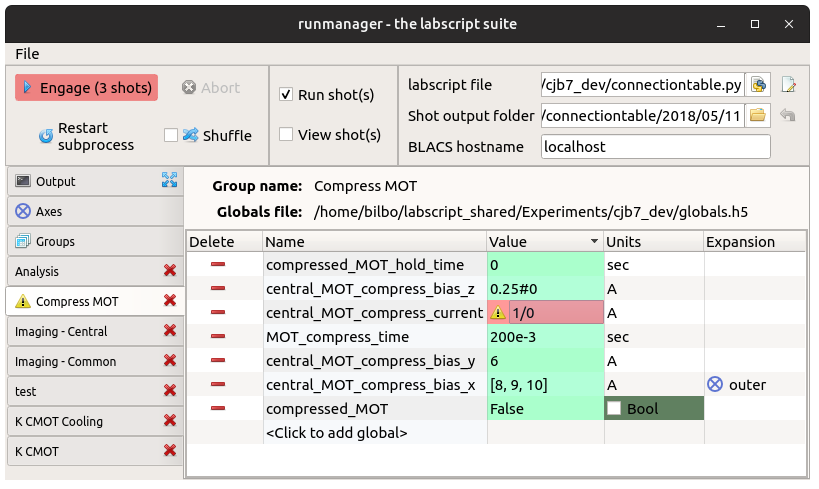
\includegraphics[width=\textwidth]{figures/software/new_screenshots/runmanager.png}
\caption{\texttt{runmanager} as of 2018, showing the interface for entering `globals', so called because they appear to the user's code as global variables. Boolean globals can be turned on and off with a checkbox, and expressions resulting in an error are highlighted in red. The `expansion' column is where the user specifies whether a global should be considered a list of values to loop over, re-running the experiment each time, and if so if that loop should be combined with other such globals to loop over the resulting product space (`outer') or whether the globals should be looped over together (`zip'\protect\footnotemark). Zipped globals can be grouped together by typing a name in the expansion column to identify which `zip group' the global belongs to. Globals in the same zip group will loop together, and multiple zip groups will form separate axes of a product space. Globals can be entered as Python expressions, including expressions containing the names of other globals. The evaluated result of an expression, or the error message if it could not be evaluated, is displayed on mouse-over for each global.}\label{fig:runmanager}
\end{center}
\end{figure}

We\footnotetext{The term for this operation---called `convolution' in computer science---comes from the name of the function in a number of programming languages for converting a tuple of sequences into a sequence of tuples. The Python \texttt{zip()} function is commonly used with sequences such as \texttt{numpy} arrays for this purpose.} refer to the process of passing the \textsc{hdf5} file to the user's code and running it as `compilation', and the resulting \textsc{hdf5} file containing both globals and hardware instructions a `compiled shot file'. Compilation occurs in a separate process from the \texttt{runmanager} graphical interface, allowing a clean separation between user code and \texttt{runmanager}, so that even the most low-level crashes of the user's code cannot crash \texttt{runmanager} and only require a restart of its subprocess. This type of separation is a repeated theme in the labscript suite and has been invaluable for making robust programs that can continue to operate in the case of inevitable crashes of user code, or of bugs within labscript suite or third-party code.

\subsection{\texttt{runviewer}}

\begin{figure}[t]
\begin{center}
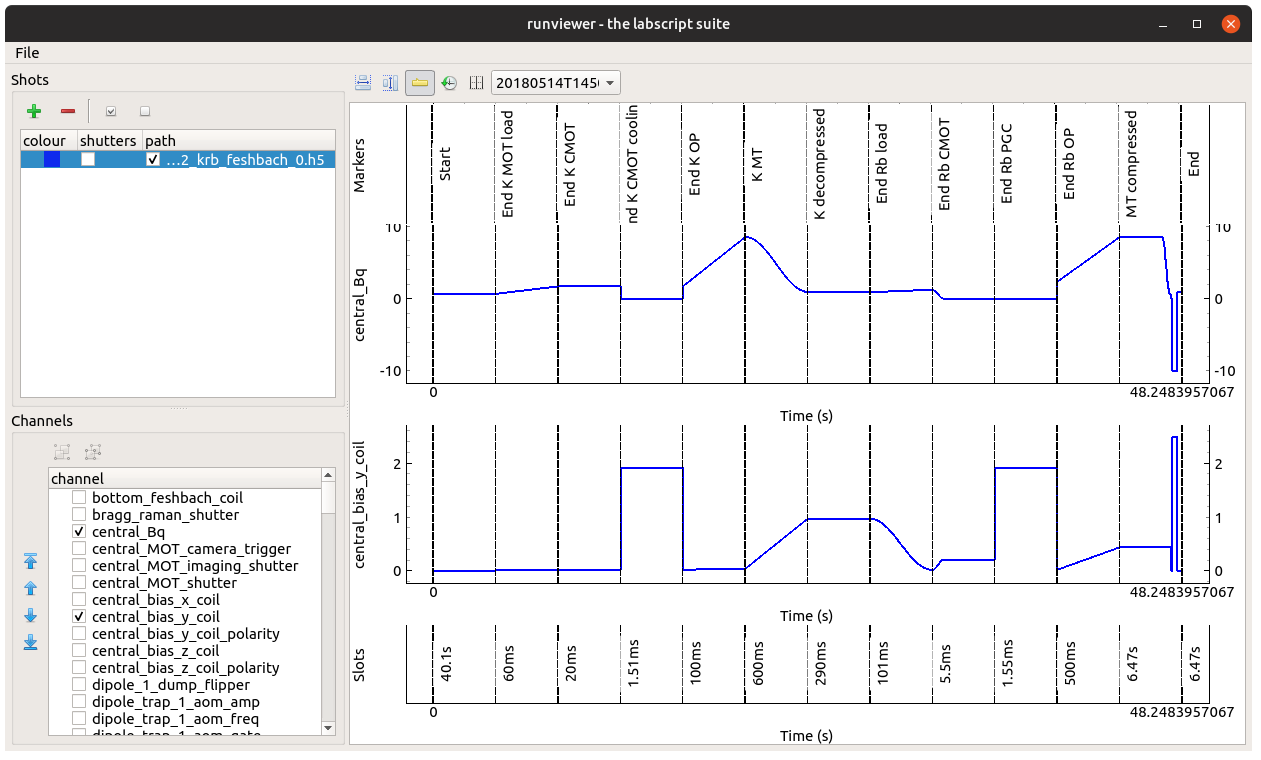
\includegraphics[width=\textwidth]{figures/software/new_screenshots/runviewer.png}
\caption{The interface of \texttt{runviewer} as of 2018, showing the recently-added `nonlinear time' feature, in which different intervals of the shot---as declared with \texttt{labscript} code---can be meaningfully shown on the same time axis in equal proportion despite being of very different duration.}\label{fig:runviewer}
\end{center}
\end{figure}

\texttt{runviewer} is a program for viewing the results of \texttt{labscript} compilation in the form of graphical plots of the voltages, digital values, frequencies etc.~that comprise the hardware instructions produced. This is useful for debugging experiment design and timing of instructions, as well as verifying that a newly made \texttt{labscript} device class (the `driver' code for each device that converts \texttt{labscript}'s intermediate description of hardware instructions into the actual format required for a given device) is functioning as intended. The \textsc{gui} of \texttt{runviewer} is shown in \figref{fig:runviewer}, illustrating the display of the output values of a number of devices varying over the course of the shot.

\subsection{\texttt{blacs}}

\texttt{blacs} (Better Lab Apparatus Control System) is a graphical program responsible for queueing experiment shots as compiled by \texttt{labscript} in tandem with \texttt{runmanager}, and executing them one after the other on the hardware. As such, \texttt{blacs} interacts with a number of Python classes that serve as \emph{drivers} for each device, containing code that uses the required software libraries, hardware drivers or communication protocols to communicate with each device. \texttt{blacs} executes the code for communicating with each device in a separate process in order to isolate them from each other, so that communication failures, software bugs, or other failures that may occur in the interactions with one device will not stop \texttt{blacs} from continuing to function in other respects. Errors are presented graphically and each device process may be restarted with the click of a button if something goes wrong, re-initialising communication with the offending device. This is useful both for responding to an unexpected failure, and for debugging when developing a driver for a new device (or new features for an existing device) to be integrated with the labscript suite.

Upon receiving an \textsc{hdf5} file from \texttt{runmanager}, \texttt{blacs} adds it to the queue of shots to be executed on the hardware. It then executes these shots in order, by programming the instructions stored in the \textsc{hdf5} file into each device, and then giving the top-level device the command to begin the experiment. Devices are programmed in parallel in their separate processes, saving time.\footnote{Particularly since many delays in programming the devices are communication delays, during which the process is simply idle.} Once the shot is complete, each device process is given the command to write any data acquired to the \textsc{hdf5} file.

\texttt{blacs} can also repeat shots, by copying and then `cleaning' an \textsc{hdf5} file after it has already run to produce a new shot file ready to be run on the hardware. It can repeat either all the shots, or just the last one in the queue. This ability to always keep running by repeating the last shot in the queue is crucial for experiments using alkali metal dispensers (`getters') or ultraviolet light-induced atom desorption~\cite{klempt_ultraviolet_2006}, as these processes must run on an approximately fixed duty cycle to maintain a stable atomic vapour pressure, otherwise experiments need to `warm up' after being idle to reach a stable pressure.

When processing of the shot queue is paused by the user or when the shot queue is empty, \texttt{blacs} remains in `manual mode', in which the devices' outputs may be controlled in real-time by the user. The graphical interface of \texttt{blacs} (shown in \figref{fig:blacs}) presents controls for the outputs of all devices, with each device and output channel labelled with its name as specified in a `connection table' file containing \texttt{labscript} code describing the connection hierarchy of all devices. \texttt{blacs} automatically generates the graphical interface for each device based a specification of its capabilities by its driver class, resulting in a set of controls for digital, analogue, and frequency generator outputs labelled with their names and using the same unit conversions set in \texttt{labscript} code for use in manual mode. Driver code may add to this interface arbitrarily to add a graphical interface for other capabilities of the device. The \texttt{blacs} queue can be paused, shots reordered or deleted, and the currently running shot can be aborted. The queue can be put in one of two repeat modes, such that either all queued shots, or only the final shot are repeated indefinitely.

\afterpage{
    \newgeometry{left=1in,bottom=1.5in,right=1in,top=1.5in}
    \begin{sidewaysfigure}[th]
    \centerfloat
    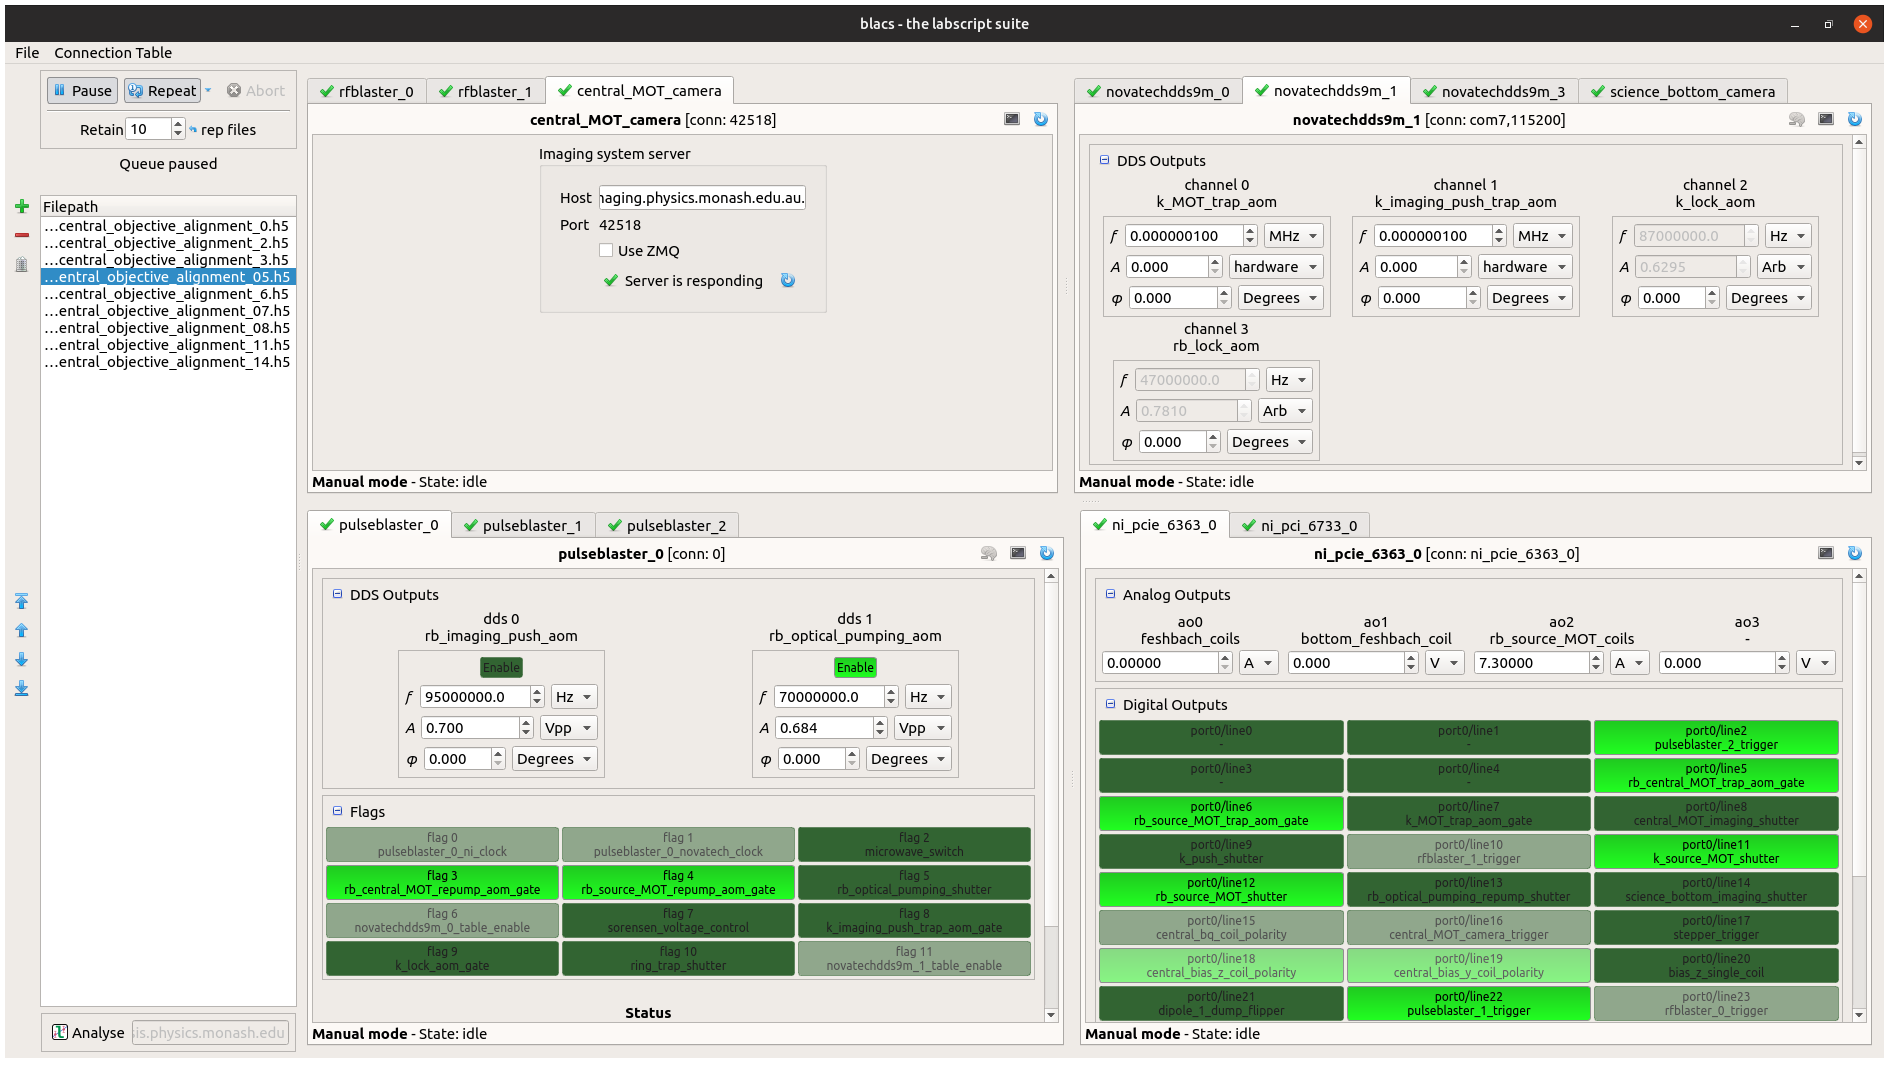
\includegraphics[width=\textwidth]{figures/software/new_screenshots/blacs.png}
    \caption{\texttt{blacs} as of 2018, showing the experiment queue to the left and manual controls of devices within a tabbed interface to the right. When a hardware-timed experiment is not in progress, outputs may be controlled manually using this interface. Presently the \textsc{gui} for four devices can be displayed simultaneously, though we plan to allow \texttt{blacs} tabs to occupy their own windows or even reside on different computers to allow a better use of screen space. Output widgets are labelled with the names of the outputs they control and can be `locked' to temporarily disallow modifications to their state. Most of the interface for each device is automatically generated from the description of the device and its outputs given in \texttt{labscript} code, though the author of a device driver for the labscript suite is free to include any graphical elements in a device tab. This screenshot was taken using the current device configuration of the Monash KRb lab.}
    \label{fig:blacs}
    \end{sidewaysfigure}
    \restoregeometry
}

\subsection{\texttt{lyse}}

Once a shot has been executed, \texttt{blacs} optionally passes the shot file on to the analysis program \texttt{lyse}. \texttt{lyse} is essentially a scheduler for user-provided analysis routines. A list of analysis routines (in the form of Python scripts), called \emph{single-shot routines} are executed in order whenever a new shot is received by \texttt{lyse}, with the shot file provided as input to each script. The analysis routines may read raw data from the \textsc{hdf5} file, or read analysis results saved by previously-run analysis routines, and save their own results. Analyis routines may also produce plots using the \texttt{matplotlib} library~\cite{Hunter:2007}---\texttt{lyse} detects these and reuses the same window for subsequent plots so that repeated runs of the analysis routines result in the plot updating in-place, rather than a proliferation of plot windows. Any other plotting library can be used (for example \texttt{pyqtgraph}~\cite{campagnola_pyqtgraph_2016}), though in this case the auto-updating behaviour is not provided automatically by \texttt{lyse}.

The shot globals and analysis results for all shots received by \texttt{lyse} are maintained in a tabular data structure---a `dataframe' provided by the \texttt{pandas}~\cite{mckinney-proc-scipy-2010} Python package---which is browsable in the \texttt{lyse} interface. This table of data is available to a further list of analysis routines, called \emph{multi-shot routines}. This list of analysis routines is also run in sequence, but only once single-shot analysis has completed on all shots presently loaded into \texttt{lyse}. These routines can be analyses of relations between input parameters and analysis results of the shots, in order to say, measure a trend of the number of atoms in a \textsc{mot} as the magnetic field gradient was varied. Both single-shot and multi-shot routines can be run from within \texttt{lyse}, or externally by running Python manually. In this latter case, the shot file on which to run single shot analysis can be provided as a command line argument, and the dataframe analysed by multi-shot routines can be obtained from a running instance of \texttt{lyse} over the network. This is no different to what happens when multi-shot routines are run from within \texttt{lyse}: they are simply run by \texttt{lyse} with no input, and are expected to call a function \texttt{lyse.data()} to obtain the dataframe containing multi-shot data. Because of the way this is implemented, one can also open an interactive Python interpreter such as IPython~\cite{perez_ipython:_2007} on any computer on the same network, type \texttt{import lyse; df = lyse.data(hostname)} (where \texttt{hostname} is the network name of the computer running \texttt{lyse}) and begin interactively exploring the data using the \texttt{pandas} library, one of its great strengths.

\afterpage{
    \newgeometry{left=1in,bottom=1.5in,right=1in,top=1.5in}
    \begin{sidewaysfigure}[th]
    \centerfloat
    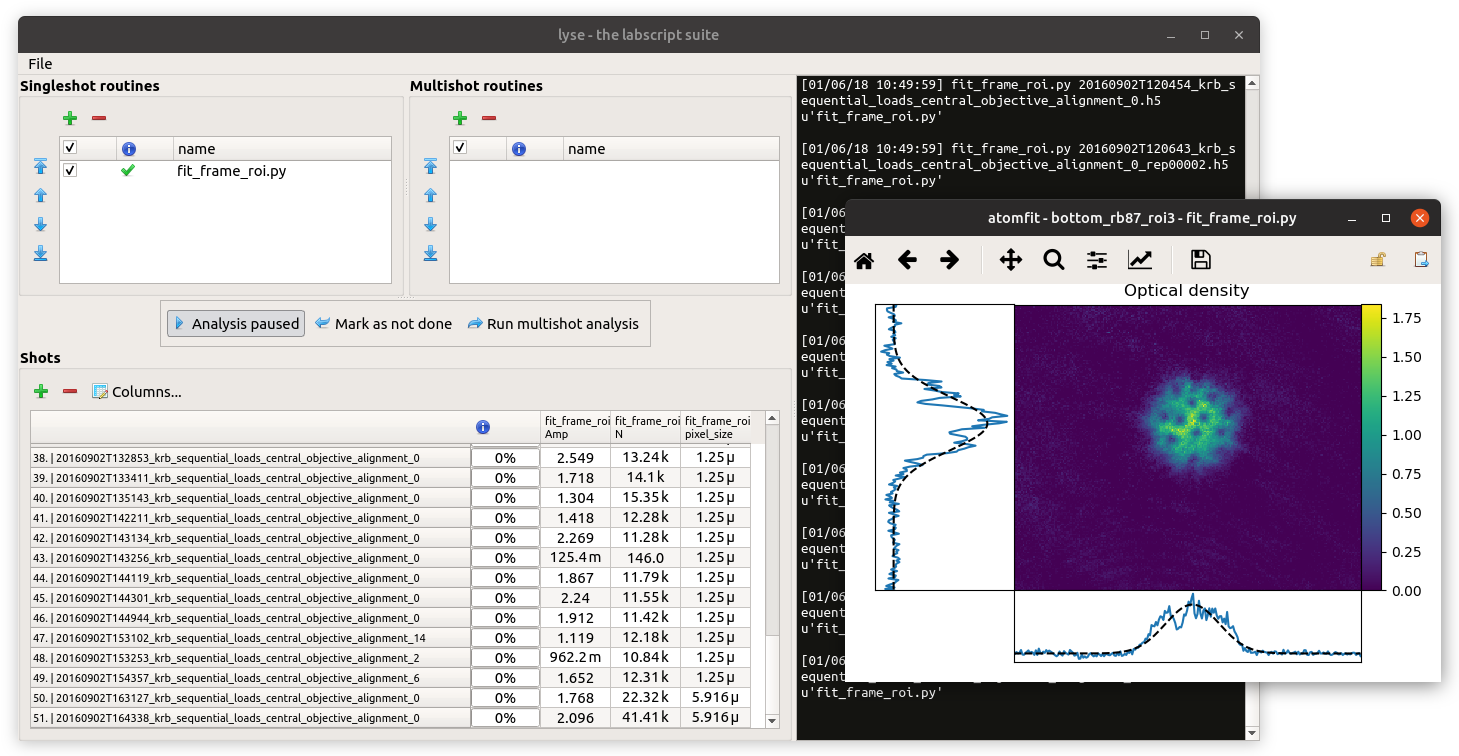
\includegraphics[width=\textwidth]{figures/software/new_screenshots/lyse.png}
    \caption{\texttt{lyse} as of 2018. To the top left is the list of single-shot routines, and to the right of it the multi-shot routines presently loaded (empty in this example). The list of shots is below them, showing some of the globals and analysis results of these shots. To the right is the output box where any textual output produced by analysis routines is displayed. Overlaid is a plot produced by a single-shot analysis routine. This screenshot was taken using shot files and an analysis routine script from the Monash KRb lab's two-dimensional turbulence experiment~\cite{johnstone_order_2018}}
    \label{fig:lyse}
    \end{sidewaysfigure}
    \restoregeometry
}

\section{Design philosophy and advantages of approach}

\subsection{It's code}\label{sec:its_code}
The design of our software brings the process of experimental physics closer to that of software development, making it amenable to many of the tools and processes in use in software development such as version control, bug tracking, and textual diffs highlighting changes between versions of experiments. Both the experiment logic and the analysis routines comprise Python code that can be examined for changes using standard `diff' tools, stored in version control, or forked into multiple versions using distributed version control and merged back together again. This can allow risky changes to experiment logic or analysis code to be explored with the reassurance of being able to roll back to a known working state should the changes not prove fruitful. One exception to this `everything is code' philosophy is the globals themselves, which are stored in non-textual \textsc{hdf5} files, though we do have a tool for `diffing' them too to highlight what has changed between two globals files, or between the current set of values configured in \texttt{runmanager} as compared to a particular shot file, which is crucial in the experiment debugging process (\figref{fig:globals_diff}).

\begin{figure}
\begin{center}
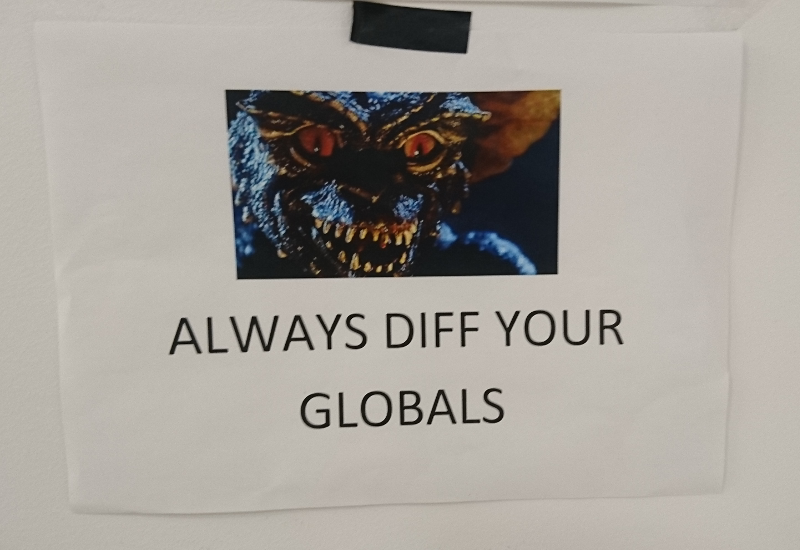
\includegraphics[width=0.5\textwidth]{figures/software/globals_diff.png}
\caption{Helpful advice from a PhD student of the Monash Spinor \textsc{bec} lab.}\label{fig:globals_diff}
\end{center}
\end{figure}

As in software development, experimental physics re-uses the same procedures time and time again, and benefits from a way to manage the complexity of turning large parts of functionality on and off, repeating them, or otherwise conditionally modifying their behaviour. In a traditional atomic physics control system, disabling or repeating a part of the experiment logic might involve tedious clicking to remove or duplicate each instruction involved. In Python, this can be a single \texttt{if} statement or \texttt{for} loop wrapping a function call containing the complexity of the part of the experiment being disabled or repeated. This ability of high level programming languages to manage complexity via encapsulation and code re-use with functions, classes and modules carries well over to experimental physics. Using an existing programming language saves us---as the developers of the control system---from having to re-invent (likely badly) the features of a programming language within our control system. For example, the tedious clicking required to disable part of an experiment in the aforementioned hypothetical `traditional' control system could be avoided if the system implemented a feature for conditionals--- akin to \texttt{if} statements. But then what about \emph{nested} \texttt{if} statements? To support all the use cases that may arise, one would ultimately be inventing and embedding a complete programming language within such a control system. Use of an existing complete (and well-designed) programming language obviates this need.

The use of an existing programming language for experiment control floe only aids the labscript suite in the case of `compile-time' conditionals and other control statements---those that can be evaluated when the hardware instructions are produced by \texttt{labscript}---as opposed to those at `run time' when the experiment is run on the hardware (such as conditionally turning a laser on if a photon is detected on a photo-detector). Such run-time control statements do require special treatment in \texttt{labscript}, and \texttt{labscript} currently only has one type of functionality like this built-in. This is the ability to pause the experiment until a pulse is produced that resumes the `master' pseudoclock. This allows the common use case of synchronisation with the background $50$ or $60\unit{Hz}$ magnetic noise from mains electricity by pausing the experiment until a fixed point in the $50\unit{Hz}$ cycle to ensure the magnetic field is close to identical from one shot to the next. It also allows servoing of the \textsc{mot} load, by loading for a variable amount of time based on a threshold fluorescence such that variations in \textsc{mot} loading efficiency from one shot to the next do not result in variations in actual atom numbers.

Further run-time control flow tools such as conditional branches would not be too difficult to incorporate into \texttt{labscript} in the future, but would require hardware capable of holding multiple alternative sets of instructions in memory and able to switch between them on a digital edge or the state of a digital signal on some input. The SpinCore PulseBlaster---the device used by most users of the labscript suite to produce clocking pulses---supports this, but most output devices labs use with the labscript suite do not. Custom field-programmable gate arrays (\textsc{fpga}s) implementing this functionality however for digital or analogue output could be integrated with the labscript suite for this purpose, as they have been for other purposes~\cite{gill_optical_2016}.

\subsection{Modularity and the Unix philosophy}\label{sec:unix_philosophy}

An aspect of the Unix philosophy~\cite{gancarz_unix_1995} is that tools should `do one thing and do it well'. The components of the labscript suite are not as minimal as they could be, but are nonetheless discrete components that encapsulate different concerns and communicate with to each other over network connections.\footnote{This is in violation of another part of the Unix philosophy that says programs should exchange text streams: our programs mostly exchange messages over network sockets, containing filenames pointing to \textsc{hdf5} files on a network drive.} Thus in principle once can remove a component and replace it with another that plays a different role. For example, \texttt{runmanager} has been re-purposed by Philip Starkey~\cite{starkey_thesis_2018} to generate parameter space scans for numerical simulations instead of experiments, by calling code other than \texttt{labscript} code. \texttt{lyse} is in use by Fred Jendrzejewski's group at Universit\"at Heidelberg for on-line analysis of experiment results in the form of \textsc{hdf5} files produced by a different data acquisition system.

The separate programs of the labscript suite are also implemented in many cases as a number of sub-components exchanging instructions over network sockets, even though the collection of processes semantically comprise a single application. This architecture facilitates a fairly direct extension (currently in development) in which different parts of the same program can be run on different computers. One can then imagine having \texttt{lyse} analysis routines run on a remote computer (perhaps a server with a powerful \textsc{gpu} or many \textsc{cpu} cores for computationally intensive analyses), or having devices controlled by \texttt{blacs} be connected to a different computer than the one running \texttt{blacs}. This latter configuration will allow blacs to simultaneously control devices that cannot be connected to the same computer; for example, those which require different operating systems or have other conflicting software or hardware configurations.\footnote{A pertinent example is the bandwidth of a computer's \textsc{usb} bus being the limiting factor in the speed at which one lab can run experiments: using two computers to program two \textsc{usb} devices could halve the programming time between shots. This is a limiting factor in the speed of experiments in the Spielman group's RbLi lab at the Joint Quantum Institute.}. The ability to control devices via additional computers that are located close to the devices they control will also reduce the need for long signal cables that can contribute to ground loops.

As mentioned earlier, \texttt{runmanager} is a graphical program, but also a software library for setting globals and compiling shots by running \texttt{labscript} code, and so is in a sense two separate components. As a result, it is possible to write code that produces shots based on something other than the simple parameter space scans \texttt{runmanager} is capable of producing. In the past, the labscript suite contained a program called \texttt{mise}, used for performing optimisation of the experiment. \texttt{mise} would use the \texttt{runmanager} library (but not the graphical interface) to produce shots based on a genetic algorithm and the results of analysis communicated to it by \texttt{lyse} analysis routines. This type of optimisation was powerful but inflexible, and we no longer maintain \texttt{mise}. However a similar method is used in the Spinor \textsc{bec} lab at Monash to integrate the \textsc{mloop} machine-learning optimisation library~\cite{wigley_fast_2016} with the labscript suite for experiment optimisation.

The separation of components also aids in development of the labscript suite. Programs can be ported one-at-a-time to use updated versions of libraries, and tested separately, enabling a more flexible model of development which has proved invaluable to the open-source development process. 


\subsection{Off-the-shelf hardware}

The labscript suite is the software part of an experiment control system, and does not mandate any particular hardware. Whilst drivers for a range of off-the-shelf and in-house devices are developed and maintained by myself and the other labscript suite developers, if one wants to use different hardware, whether off-the-shelf or custom, one can write drivers for it and use it with the labscript suite. This does mean that the software cannot make hard assumptions about the hardware and has to deal with a wider range of possibilities, which is a complicating factor in maintaining the code, but I believe this approach is the better one compared to designing a limited range of hardware specifically for the labscript suite or vice versa. It is difficult to anticipate what hardware capabilities experimentalists will require for atomic physics experiments in the future, and science is by its nature pushing the envelope such that converging on `standard' hardware can be at odds with making scientific progress. Therefore it is better to leave the software as agnostic as reasonably possible when it comes to hardware.

Labscript suite developers and users have also made some hardware of their own, and there exists a low-cost pseudoclock and a digital out device both based on a sub-\$100 microcontroller board (Called the PineBlaster and BitBlaster respectively). However these have proved difficult to maintain in the face of changing software development kits for the microcontrollers, and I suspect \textsc{fpga}s implementing similar functionality would be a solution with greater longevity. Rory Speirs~\cite{speirs__2018-1} has developed a low-cost \textsc{fpga}-based pseudoclock (planned to be released as an open-source project) that may be an attractive alternative to the SpinCore PulseBlaster for use with the labscript suite.

\subsection{Open-source, popular programming language and data format}

Using open-source technologies in the labscript suite, as well as developing the labscript suite itself as an open-source project have benefited the project considerably.

The labscript suite itself being open source allows others to modify it to their needs, expanding the range of experiments that it can be used with. If modifications made are applicable to a wide enough range of users, they can be contributed back to the main project. Not least importantly, bugs in the code that have been worked around or fixed by a single end-user can be contributed back to the main project for the benefit of all. This has led to a steady improvement in the usability and stability of the software as usability issues and bugs have been noticed and fixed by people inside and outside the core development team. Sometimes there is disagreement about what features belong in the labscript suite, or more often, over how they should be implemented. The open-source nature of the project allows end users to continue to use an implementation of functionality that there may not be agreement about including in the main project, either permanently or until another implementation is available. This is preferable to simply being at the mercy of the core developers as to what features they will or will not implement (whether due to differing opinions or to time constraints).\footnote{Although a commercial model has the potential to to work here too, in which users pay for features to be implemented. There is also the `best of both worlds' approach of bug and feature `bounties', where users add a cash reward for implementing certain features or resolving bugs, adopted by some open-source software projects.}

The use of third-party open-source technologies in the labscript suite has also been advantageous, as when the projects we rely on do not fully satisfy our needs, there is often the possibility of modifying them to meet those needs. Furthermore, these modifications, if agreeable to the developers of said libraries, can be included in the `upstream' project to remove the requirement that we maintain the patches ourselves. To this end I have had changes accepted into the \texttt{numpy}~\cite{oliphant_guide_2015}, \texttt{pandas}~\cite{mckinney-proc-scipy-2010}, \texttt{pyzmq}~\cite{brian_e._granger_and_contributors_pyzmq_2018} and \texttt{h5py}~\cite{andrew_collette_and_contributors_h5py_2018} projects which improve their behaviour for the labscript suite's purposes. 

The use of a popular programming language with a gentle learning curve such as Python allows new students writing experiment code using \texttt{labscript} to get up to speed with what is necessary to work in their laboratory quickly compared to other programming languages. Many students and other physicists are already using Python for data analysis and other tasks, and so knowledge of it is more widespread than other languages, decreasing the barrier to entry for modifying the labscript suite or contributing to its development.

The use of the standardised \textsc{hdf5} format, and of the popular \texttt{zeromq}~\cite{zeromq_guide} messaging protocol for communication between components allows interoperability with a wide range of other programming languages and technologies, such that software written in other programming languages can interact with running labscript suite programs and read the data files produced by them. The camera interface program \texttt{BIAS} mentioned earlier is an example of this---it is written in LabVIEW and yet reads and writes data to the same shot files as the rest of the labscript suite using the \textsc{hdf5} library, and communicates with components of the labscript suite over the network using the \texttt{zeromq} library.


\subsection{Collateral benefits}

Developing and maintaining the labscript suite has involved achieving several intermediate, instrumental goals in order to achieve the ultimate goals of the software. Some of these solutions have been packaged as separate software projects, or are available from within the labscript suite, and may be used for other purposes.

For example, as mentioned, the labscript suite comprises several programs, each of which contains multiple threads and/or processes, communicating with each other by message passing (largely in line with the `actor model' of concurrent programming\footnote{Though we had no formal education in this model before writing code in this style, and I attribute my fondness of the model to the computer game \emph{SpaceChem}~\cite{zachtronics_industries_spacechem_2011}, in which the player constructs chemical `reactors' comprising multiple threads of execution exchanging atoms and molecules.}). As such the code contains reusable pieces for launching processes and initiating message passing with them, of redirecting output of subprocesses to some visible location rather than a terminal, or of starting and stopping `servers' and creating `clients' to either pipe data continuously or make discrete requests that necessitate a response. Furthermore, these multiple threads and processes often require access to the same files (the \textsc{hdf5} files containing the data for each experiment run), and access to these files needs to be serialised to prevent data corruption, including the case of multiple computers attempting to access the file over the network. The solutions to these problems that we have arrived at are encapsulated into the \texttt{zprocess} project~\cite{billington_zprocess_2018}, an open-source software project officially separate from the labscript suite but very much developed to meet its needs for multiprocessing. This project is used not just for the labscript suite, but for other laboratory automation tasks. It is also used in the software implementation of an undergraduate experiment in the School of Physics and Astronomy at Monash University to allow students to remotely control the experiment and collect data over the internet~\cite{monash_university_school_of_physics_and_astronomy_measurement_2016}.

Multi-threaded graphical programs can present development problems as the software library for the graphical interface generally must be accessed only from the one thread. This is generally the case for the Qt toolkit~\cite{the_qt_company_qt_2018} as used in the labscript suite, and so interacting with the graphical interface from multiple threads generally involves message passing to request that an operation be performed in the `main' thread. We have similarly encapsulated our solutions to this---as well as several other problems repeatedly encountered in using the Qt toolkit, such as an icon set, automatic loading of graphical layouts from external files, and others---into the \texttt{qtutils} project~\cite{starkey_qtutils_2018}, which is used for other small graphical utilities in our group, separately from the labscript suite. This library has also been used in an undergraduate teaching context in the School of Physics and Astronomy at Monash University to improve IT infrastructure for digital logbooks used by undergraduate students.

We also have a number of debugging/profiling tools that I often find myself reaching for to debug numerical simulations, or other code unrelated to the labscript suite.


\section{Recent and future developments}

Since the publication of our paper in 2013~\cite{starkey_scripted_2013}, the number of groups using our software has increased considerably, from being limited to just the two groups at Monash, to a modest number of groups around the world.

In 2014 during my PhD I was invited to visit the Joint Quantum Institute in the group of Ian Spielman, with the aim of improving the labscript suite to make it more generally usable and easier for others to install. The primary goal was to port the graphical programs from the \textsc{gtk} toolkit~\cite{the_gnome_project_gtk+_2018} to the Qt toolkit~\cite{the_qt_company_qt_2018}, and to write an installation program that would automate the previously somewhat tedious installation process. These goals were achieved, and the installation process for the labscript suite is now a matter of installing an appropriate Python environment, and then downloading and running our installation script.

The following subsections detail this and a number of other developments since the publication of our paper, as well as planned and in-progress improvements to the labscript suite.

\subsection{Port to Qt}

The port to Qt~\cite{the_qt_company_qt_2018} was a crucial development. As discussed in the publication reproduced at the end of this chapter, we initially chose the \textsc{gtk} toolkit for its cross-platform compatibility and good Python bindings~\cite{riverbank_computing_pyqt_2018}. This proved to be the wrong decision, as the \textsc{gtk} project has rapidly developed and dropped support for older versions, with the newer versions being difficult to install or deploy on operating systems other than Linux, and with changes being significant enough to impose a considerable ongoing development cost to keeping code up to date with them. Although slated as a cross-platform toolkit, the \textsc{gtk} project is developed by and primarily serves the needs of the \textsc{gnome} project~\cite{the_gnome_project_gnome_2018}, and thus its development is driven by those needs. There is little incentive for Windows- or Mac-specific bugs to be fixed, or for the installation process to be improved. Although it's an open-source project such that people other than the core developers could contribute fixes to these issues, the Linux-centric nature of the project impedes these fixes from being accepted for inclusion. Switching to the (also open-source) Qt toolkit is the chosen solution for most for cross-platform graphical software, and so this is what we have now done as well. The experience of both maintaining and installing the labscript suite is much improved as a result. Being the standard cross-platform \textsc{gui} toolkit, Qt is already available in the standard Anaconda Python distribution~\cite{continuum_analytics_anaconda_2018}, which is the preferred Python distribution among scientists at the present time. With our \texttt{qtutils} package, an icon set is available, obviating the need to install a separate icon pack as was previously the case. Most importantly, the Qt software project exists to serve the needs of graphical programs generally, and is used by many major cross-platform projects. Combined with the fact that Qt is open source, this is insurance against future breaking changes in Qt or against the Qt Company going out of business---open source projects can be forked and maintained by the community, and the more popular they are the more likely this is to occur if they take an unpopular turn or are abandoned by their present maintainers. We therefore have confidence that the Qt project's direction is aligned with the needs of the labscript suite, and that we can continue to rely on it in a way we could not with the \textsc{gtk} project for our project's longevity without introducing unnecessary technical debt.


\subsection{Python 3}

The labscript suite was initially written in version 2.7 of the Python programming language, even though version 3 of Python had been released several years prior. The Python community has in this time been in a decade-long transition from one version to the next due to some non-trivial differences between the two versions of the language. I believe we made the right decision to initially use Python version 2.7, as many of the technologies the labscript suite relies on did not have Python 3 compatibility for some time. However, the point of inflection in the adoption curve for Python 3 has occurred in the last two years or so, and now is the right time for Python 3 adoption. With the help of third party contributors (primarily Jan Werkmann), the entirety of the labscript suite has now been ported to run on both Python 2 and Python 3, though we do not consider the support `official' until more testing has been performed, particularly using hardware not in use by the groups that are running with Python 3 daily.

We do not expect such an extended issue such as this to occur again: the Python core developers consider this transition to be a one-off, and future porting efforts of labscript-suite components will likely be no more work than the usual required to keep up with minor changes between language versions.

\subsection{More devices, more features, general polish}

There are more devices with compatibility with the labscript suite, and more models and features of existing devices are now supported. The programs are easier to use, and many cases where obscure errors were thrown have been replaced with friendlier error messages explaining the situation in human-readable terms. Following is an incomplete list of minor to modest usability improvements:

\begin{itemize}
    \item \texttt{blacs} now has a plugin to delete shots that are repeated versions of previous shots. This prevents unnecessary consumption of disk space when these shots are running only to keep an experiment `warm' (initially implemented by Ian Spielman, and re-implemented by me as a plugin for \texttt{blacs}).
    
    \item \texttt{lyse} now more gracefully handles shot files that have been deleted off disk: declining to run single-shot analysis on them, but keeping their data in the dataframe available for multi-shot analysis until they are deleted from the \texttt{lyse} interface. This aids in, for example, diagnosing a day-long drift in some performance characteristic of the experiment even though most shot files are deleted due to the aforementioned desire to save disk space (implemented by me).
    
    \item \texttt{lyse} is now more performant, only updating those values of the dataframe that have changed, and minimising the number of times it opens a \textsc{hdf5} file. This improves performance for very large numbers of very short duration shots, as is common in ion trapping (implemented by Jan Werkmann with changes by me).
    
    \item \texttt{blacs} has had some bugs resolved that unnecessarily introduced delays on the order of $0.5\unit{s}$ in between running shots. These delays were not very noticeable for the cold atom experiments of order $15\textrm{--}30\unit{s}$, but again are important for the ion trappers (implemented by me and Philip Starkey).
    
    \item \texttt{blacs} tabs now have a separate optional terminal output for each device subprocess, allowing simpler debugging and development of devices (implemented by me).
    
    \item More flexible camera interface. There are now a number of camera `servers' in use by various groups playing the role that \texttt{BIAS} plays at Monash, including a fork of \texttt{BIAS} named \texttt{unBIASed} by Ian Spielman (changes made to facilitate communication with Python camera servers implemented by me)
    
    \item \texttt{labscript} can now accept arbitrary function ramps using user-supplied functions, not limited to the built-in list of functional forms. This has always been possible somewhat manually, but now has a more friendly interface (implemented by me).
    
    \item There is now a unified interface for saving and retrieving configuration settings of devices in \texttt{labscript} to the \textsc{hdf5}, including Javascript Object Notation serialisation for complex data types that do not coincide with a \textsc{hdf5} datatype. This replaces a number of ad-hoc serialisation methods previously in use to store configuration settings of devices (specification designed by Ian Spielman and core developers, implementation by Ian Spielman and me).
    
    \item There is now a unified \texttt{labscript} device driver for National Instruments DAQmx devices, removing the code duplication and complexity of maintaining multiple device classes for this range of devices. This class exists in the fork of the \texttt{labscript\_devices} repository in use by the Spielman group at the Joint Quantum Institute, but will be merged into the mainline codebase soon---it is already in use by groups who are not otherwise using the Spielman fork of the code, and so has undergone some testing and bugfixes outside of the hardware in the Spielman group. In time the model-specific code will likely be removed in favour of the unified interface (implemented by Ian Spielman).
    
    \item The ability to mark certain points in time of the experiment with a named marker, visible in \texttt{runviewer} to visibly delineate different stages of the experiment (implemented by Jan Werkmann).
    
    \item A `nonlinear time' mode for runviewer, where the time axis is not linear but instead uses a different timestep for the different stages of the experiment as described by the markers. This allows short timescales and longer timescales to be visible on the same plots in \texttt{runviewer}. (implemented by Jan Werkmann with changes by Shaun Johnstone).
    
    \item The ability to mark digital outputs as `inverted', such that digital low represents a device being on, semantically speaking. The buttons for these outputs are represented with different colours in the \texttt{blacs} interface to avoid confusion (implemented by Jan Werkmann).
    
    \item Gated clocks: devices with vastly different memory capabilities can receive clocking signals from the same clocking device such as a PulseBlaster, but on different outputs such that the clock ticks intended for one device are not received by other devices. There is still a single pseudoclock, but its outputs are `gated'---whilst the clock is ticking for one device it is not ticking for another. Two devices configured in this way are still however sharing a clock in a sense: they cannot both receive rapid clock ticks simultaneously but at different rates, multiple pseudoclock devices are still required for this (implemented by Philip Starkey).
    
    \item \texttt{lyse} plots can be copied to the clipboard with a button click, reducing the number of steps to include plots in a digital log book (implemented by me).
    
    \item \texttt{runmanager}, \texttt{lyse}, and \texttt{runviewer} now have the ability to save and load configuration settings, such that the same sets of globals files in the case of \texttt{runmanager} or the same sets of analysis routines in the case of \texttt{lyse} and the same view settings in the case of \texttt{runviewer} can be loaded at start-up of each application (implemented by me for \texttt{runmanager} and Jan Werkmann for \texttt{lyse} and \texttt{runviewer}).
    
    \item \texttt{runmanager} now allows finer control over parameter spaces, including randomising the order of a parameter space scan on a per-axis basis, and control over the nesting order in which the axes are looped over (implemented by Philip Starkey).
\end{itemize}

\subsection{Optimisation}

The program \texttt{mise}, mentioned in the paper, has been deprecated. Nothing has replaced it, though due to the modularity of the labscript suite, optimisation is still possible through use of the \texttt{runmanager} library directly. This is a testament to the pluggability of the labscript suite components, but could nonetheless be improved.

I plan to improve this functionality in the future, and one of the near-term development goals is to add a `remote' application programming interface (\textsc{api}) for \texttt{runmanager}. This will enable a program to control a running instance of \texttt{runmanager} to set the values of globals and initiate shot compilation and submission to \texttt{blacs}. This will be a much simpler interface as well as being compatible with just-in-time compilation, discussed below.

\subsection{Just-in-time compilation}\label{sec:jit}

One feedback mechanism not previously anticipated---more accurately described as \emph{feed-forward} in this context---is the need to modify one or more parameters for the very next shot to be run on the experiment, but otherwise remain performing some parameter space scan or repetition. For example, in the Spielman group's atom chip lab, an environmental magnetic field drift on a several hour timescale is corrected for by performing an error measurement each shot, to be fed-forward to the next shot as a change in the applied field bias. Other than this, the experiment is not performing any optimisation or feedback. In the chip lab, this functionality is implemented by having \texttt{blacs} use the \texttt{runmanager} \textsc{api} to re-compile the shot files just before running them, to be sure to include the updated magnetic field bias estimate. 

This works, and is an example of functionality being implemented by users to serve an immediate need. However I would like to move this `just-in-time' compilation into \texttt{runmanager}, so that the shot is compiled only once rather than being recompiled. Compilation by \texttt{blacs} is unappealing since it may be on a different computer with different versions of the code being compiled, leading to the possibility of subtle errors, and more generally violates the design philosophy of separation of concerns that has served us well so far. 

For this reason as well the applicability to optimisation mentioned above, I plan to implement both a remote \textsc{api} for \texttt{runmanager} as well as a `compilation queue' containing shots yet to be compiled, whose variables can still be changed (possibly remotely) up until the moment \texttt{blacs} requests a new shot,\footnote{Either because its queue is empty, or nearly empty---by requesting a shot before the queue is fully empty one can prevent the experiment being idle during compilation, at the expense of the feed-forward changes taking effect only some number of shots in the future.} triggering compilation to occur.

\subsection{Fixed duration shots}

Since \texttt{blacs} takes a usually small---but variable---amount of time to program the hardware in between shots, this contributes to a variation in the average proportion of time an atom dispenser is receiving current or ultraviolet light-induced desorption is active, leading to vapour pressure variations in experiments that operate in this manner. In the Spielman fork of the \texttt{blacs} repository, there is functionality to set a fixed overall duration for an experiment, such that after programming devices, \texttt{blacs} waits some additional amount of time such that experiments are run at precisely equal intervals. This can be used not only to smooth out the variations in programming time, but also to smooth our variations in actual shot duration caused by changes of parameters that affect the shot duration, or changes in shot duration due to variable-length waits while the experiment is paused, such as servoing a \textsc{mot} load as mentioned in Section~\ref{sec:its_code}. This feature is yet to be merged into or reimplemented in the mainline labscript suite codebase from the Spielman fork.

\subsection{Remote devices}

A work in progress is to allow devices to be connected to any computer, not just the one that \texttt{blacs} is running on. As mentioned in Section~\ref{sec:unix_philosophy}, this allows one to avoid long signal cables and their associated propagation delays and potential ground loops, as well as to make better use of limited computer resources by spreading processing over more computers. It also would allow one to make better use of computer screen real estate if the graphical interfaces for each device within \texttt{blacs} could be presented on a different computer as well, since the \texttt{blacs} interface can become quite cluttered with a large number of devices. One reason for making a separate camera control program in the form of \texttt{BIAS} was to be able to view images immediately at all times without having to ensure the correct tab in the \texttt{blacs} interface is active. Being able to display these tabs as separate windows on different screens or computers will obviate this need and allow cameras to be once again treated the same as other devices.\footnote{This was not the only reason \texttt{BIAS} was made as a separate system, another reason was the availability of software libraries for interacting with certain cameras, these were available for LabVIEW at the time, but not Python. Python wrappers, \texttt{pyvisa}~\cite{torsten_bronger_pyvisa_2018} and \texttt{pynivision}~\cite{peter_johnson_frc_team_294_pynivision_2015} for the National Instruments \texttt{VISA} and \texttt{NI-Vision} libraries have since become available, removing the need for LabVIEW to be used with cameras or other devices requiring these interfaces.}

In discussion with developers and users, we have designed a specification for how the desired layout of devices on a network will be described by users in \texttt{labscritp} code, and we have a partial implementation. Most of the work toward this has been in the \texttt{zprocess} package, which I have been adapting to these needs, including the use on encryption to ensure that the ability to start processes on remote computers is secure. This feature in \texttt{zprocess} is nearly complete, after which some work in \texttt{blacs} will need to be done to implement the designed specification and make the appropriate requests to \texttt{zprocess} to launch remote processes for communicating with hardware and displaying the graphical interfaces for them. These two features are planned to be separate, such that \texttt{blacs}, the graphical interface for a specific device, and the device itself can be on the same computer, or two, or three, for maximum flexibility in where the graphical interfaces and actual hardware is located within the lab.

\section{\texttt{labscript} version 3}

The \texttt{labscript} compiler itself is the oldest part of our codebase, and has changed significantly since its initial incarnation. We have become more skilled programmers in the $7$ years since it was first written, and some design decisions have proved to be the poorer choices. For example, most processing performed by \texttt{labscript} during processing is \emph{destructive}---that is, new data replaces old data as processing steps proceed. Specifically, timing delays are incorporated by replacing timing data in instructions, rather than introducing new variables in code specifically for the delayed timing data whilst leaving the original timing information intact. This makes it difficult to debug where timing problems have occurred, and makes the code fragile to the introduction of bugs in which timing offsets are accidentally taken into account twice or not at all, as opposed to exactly once as required. Furthermore, these timing calculations are performed mostly using floating point arithmetic, and so all comparisons need to be performed with some tolerance or rounding. This is error-prone and unnatural given that the hardware devices generally have quantised timing in their instructions. Finally, by the time an exception occurs in \texttt{labscript} indicative of the user requesting something not possible (such as two instructions closer together in time than the hardware is capable of), \texttt{labscript} no longer has much information about where in the user's code the instruction originated, making it difficult to give the user information that helps them resolve the issue.

To address these three concerns, I have been working on an experimental restructuring of the core instruction and timing processing of \texttt{labscript}, in which all processing is non-destructive, the points in the user's code where instructions are created are noted for later use in error messages, and all timing calculations are performed using integer arithmetic after quantising timing details as early as possible in processing according to the time resolution of the pseudoclock controlling the timing of each device. This project, called \texttt{labscript\_core}, if successful will eventually replace the part of \texttt{labscript} responsible for timing calculations and instruction handling, making the code better from both the perspectives of users and developers. If possible I will keep the timing computations separate from the other higher level parts of \texttt{labscript} (globals, device properties, \textsc{hdf5} files) so that it can be independently tested (ideally in the context of an automated test suite) and verified so that we can have a high degree of confidence in the output it produces, and confidence that regressions have not been introduced when changes are made.


\section{Other future developments}

A pressing concern is to unify the mainline labscript suite code with the Spielman group's fork of the code. This will involve merging (or re-implementing in the mainline codebase) the remaining features present in the Spielman fork as discussed in the previous sections, as well as others I have not mentioned such as a progress bar showing the progression of the experiment, and the ability to insert small analysis scripts to be executed by \texttt{blacs} at the end of a shot with the sole purpose of updating parameters in \texttt{runmanager} for feed-forward functionality as described in Section~\ref{sec:jit}.

There are a number of 3rd party contributions (mostly authored by Jan Werkmann) awaiting approval by a core maintainer such as myself or Philip Starkey. Some of these are:
\begin{itemize}
    \item Analog input widgets for \texttt{blacs}: these show a numerical value for the voltage of each analog input a device has, or optionally can display an interactively updating plot of the voltage trace over time.
    \item Plugin tabs for \texttt{blacs}: this allows plugins for \texttt{blacs} to insert tabs into its graphical interface, allowing plugins to have rich interfaces of their own without having to interfere with the main interface of \texttt{blacs}
\end{itemize}

Other changes proposed but not implemented include:

\begin{itemize}
\item `Analysis globals': like the globals set in \texttt{runmanager}, but set in \texttt{lyse} instead. Presently, users are `abusing' globals set in \texttt{runmanager} in order to configure how analysis will run. For example, there are globals being set by users that tell analysis code which pair of variables to plot against each other. As this may change after a shot has run, an interface where `analysis globals' can be set and used by analysis routines would be preferable.
\end{itemize}

Finally, the entire project would benefit from more and better documentation. Documentation exists,\footnote{Primarily written by Philip Starkey}, though it could be more thorough, and more importantly the development process has not ensured that documentation keep up to date with changes to the code. Instead, new information is often hidden in comments within the code or in commit messages. I see this as a flaw in the development process, rather than one of lack of effort or consideration. The Python community has a solution to this problem, which is to use libraries that turn appropriately formatted code comments into proper documentation. This then creates incentives to write and update these comments to a higher standard, knowing that they will be visible in official documentation---and this standard is more likely to be enforced during code reviews that occur when pull requests are made for changes to be included in the mainline code repository. Such a change of process would help maintain and improve documentation continuously over time, and is better in my opinion than occasional bursts of effort and re-writes of the documentation.

In light of the existing open-source development model, an effective strategy to implementing a change such as this is to sow the seeds what we would like to see by putting the documentation rendering mechanism in place despite the current inadequacy of the documentation contents, and then require that contributions (from core developers or otherwise) in future amend the documentation comments (called `docstrings' in Python parlance) appropriately. This way over time the documentation will improve, and being code rather than a \textsc{pdf} or Microsoft Word document, be amenable to pull requests and bug reports in the same manner as the rest of the code, which we have seen leads to inexorable improvement via an open process that accepts external fixes from others.

There is also a substantial quantity of best-practices and lore built up about hardware as well as software, including many tips and tricks that are specific to certain setups. Whilst the labscript suite has a mailing list in which much of this information is exchanged, it would probably benefit the project to have a user-editable wiki, to decrease the barrier-to-entry for users to share this type of domain-specific knowledge outside the context of an email thread even though it may not suit the official project documentation.

\section{Project history and attribution}

\begin{figure}
    \centering
    \subfloat[]{
    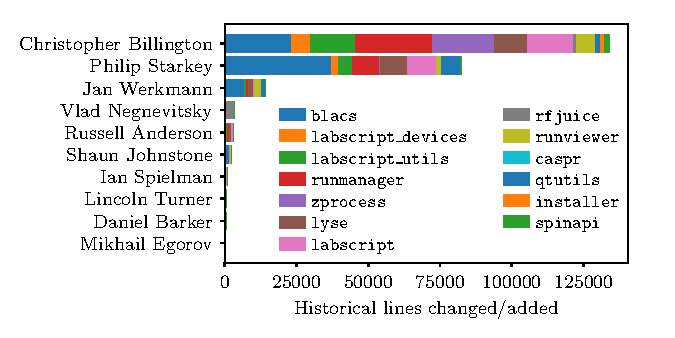
\includegraphics{figures/software/churn.pdf}
    }\\
    \subfloat[]{
    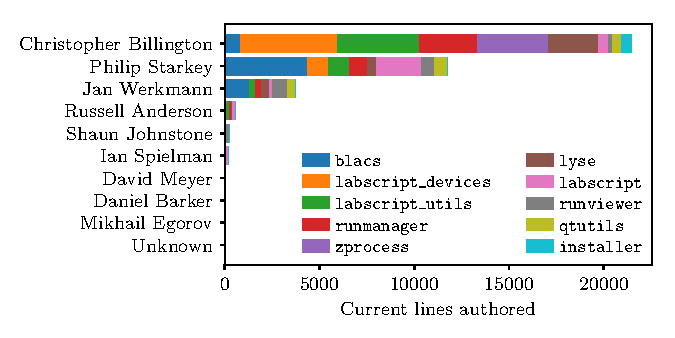
\includegraphics{figures/software/blame.pdf}
    }
    \caption{Authorship by lines of code of each component of the labscript suite, for the top ten authors. (a) Authorship of line changes over the entire project history. (b) Authorship of lines currently present in the most recent revision of each component. The line counts for these plots were obtained using the mercurial `churn' extension and `blame' command to analyse all Python, Cython and C source files in our code repositories. This excludes documentation (most of which is in Microsoft Word format) as well as layout files for the graphical interfaces of the programs. Although these results are broadly representative of authors' contributions to the components of the labscript suite, they should be taken with a grain of salt. Authorship is difficult to ascertain programatically as refactoring counts the same as original authorship even though usually less credit (though not zero) should be assigned to someone refactoring code than the author writing it originally. As such my apparent contribution to \texttt{labscript\_devices}---the repository containing device drivers---is exaggerated due to me being the one to migrate this code from another repository. Similarly Jan Werkmann's contributions to \texttt{blacs} are exaggerated due to recent renaming of one particular large source file. We both have made original contributions to both repositories as well, but these are not distinguishable from refactoring in these plots. The three repositories \texttt{caspr}, \texttt{rfjuice} and \texttt{spinapi}---not previously mentioned in this chapter---are libraries for interacting with devices, the former two for the `RFBlaster', an \textsc{rf} synthesiser designed and built by Vlad Negnevitsky and used at Monash University and the Australian National University~\cite{altin_precision_2013}, and the latter for the SpinCore PulseBlaster, in use by most groups using the labscript suite.}\label{fig:line_counts}
\end{figure}

This section acknowledges the contributions of different authors to the different components of the labscript suite, and provides a history of major developments. This is not comprehensive, and many improvements have been provided by others; nonetheless the majority of the design and programming effort behind the labscript suite is due to the authors responsible for the initial creation and major developments of each subproject as outlined below. A full history of the codebase is publicly available on our on-line version control repositories~\cite{monash_univeristy_labscript_2018, starkey_qtutils_2018, billington_zprocess_2018} and can be used to credit any particular change or piece of code to the appropriate author.\footnote{With the exception of generic usernames occasionally being used from lab computers such that authorship was not recorded.} Plots of present and historical authorship by number of lines of code are shown in~\figref{fig:line_counts}.

The initial idea of having object-oriented Python code compiled to low-level instructions was inspired by a similar implementation by Scott Owen and David Hall~\cite{owen_fast_2003} in which experiment logic is described in C++ and programmed into the hardware using a LabVIEW program with a state-machine architecture.

Toward this goal I developed an initial implementation of the \texttt{labscript} compiler in Python in February 2011, subsequently improving it over time. Throughout the following year or so, the architecture of the software suite, its components and how they would interact was developed by members of the Monash Quantum Fluids group including Lincoln Turner, Russell Anderson, myself, Philip Starkey, Shaun Johnsone, Martijn Jasperse, and others.

The initial implementation of programming the \texttt{labscript}-generated instructions into hardware in LabVIEW was due to Russell Anderson in early 2011, followed by the initial version of \texttt{runmanager} written by me in August 2011 and the initial version of \texttt{runviewer}, also by me, in September 2011. Early in development I moved \texttt{runviewer} to use the Qt toolkit in order to take advantage of the \texttt{pyqtgraph}~\cite{campagnola_pyqtgraph_2016} plotting library, which was necessary for acceptable performance of \texttt{runviewer}.

Philip Starkey wrote the initial version of \texttt{blacs} in October 2011, superseding the LabVIEW control system. In November 2011 Philip Starkey and I re-architected \texttt{blacs} to move to a multi-process model (it was previously only multi-threaded) and improve the state machine architecture it uses.

In February 2012 I wrote \texttt{lyse}. In April 2012, Philip Starkey re-wrote a substantial portion of \texttt{runmanager}, making its user interface suitable for larger number of globals and improving other functionality.

In January 2013, Philip Starkey ported \texttt{blacs} to use the Qt toolkit.

In May 2014, Philip Starkey expanded the capabilities of the \texttt{labscript} compiler by implementing the `gated clocks' feature, allowing more devices to be controlled by a single pseudoclock device such as a SpinCore PulseBlaster. Between August and November 2014 while visiting Ian Spielman's group, I ported \texttt{runmanager} and \texttt{lyse} to the Qt toolkit, wrote the labscript suite installer script and adopted the practice of tracking dependencies of the different components on each other using semantic versioning.

Throughout this time device driver code was contributed, various features implemented and bugs fixed by many, including Russell Anderson, Shaun Johnstone, Martijn Jasperse and Ian Spielman. Documentation was written primarily by Philip Starkey. \texttt{BIAS} was written and maintained by Martijn Jasperse from late 2011 onward.

When we started writing applications in Qt, I wrote the initial code for multithreading in Qt that became the \texttt{qtutils}~\cite{starkey_qtutils_2018} package, with most of the later functionality in the package added by Philip Starkey.

The \texttt{zprocess} package, encapsulating the network communication and multiprocessing code common to several components within the labscript suite, was written and is maintained by me (as always with some bugfixes and features contributed by others).

\section{Conclusion}

The labscript suite is an increasingly mature software project for control of hardware-timed experiments. It has an increasing number of users and contributors, and has evolved to keep up with changing software environments in the sense of switching to use more dependable software libraries such as the Qt \textsc{gui} toolkit, and of keeping up with updates in language and library changes, such as the shift to Qt version 5 and to Python 3. It is a living project accepting changes from non-core developers, and is free for anybody to use under a permissive license. Due to the modular design and open development process, the labscript suite has thus far avoided some of the pitfalls that befall many laboratory control systems and software, such as relegation to legacy software or hardware environments due to a lack of development process capable of keeping them up to date, or long-standing bugs not being resolved because a fix applied in one place has no mechanism of making it into other users' installs of the software, or because the source code is only understood by or available to a small few. The labscript suite is hardware-agnostic, ensuring its use is not restricted to officially sanctioned or in-house hardware. Finally, it is written in a very popular programming language with an abundance of on-line resources and a vibrant community behind it, within both scientific and software engineering circles. Rather than the implementation details of the code itself, it is these decisions that I think are causing the project to thrive and be as beneficial to experiment physics research as it has so far.

\section{Reproduced publication: A scripted control system for autonomous hardware-timed experiments}

See over page for a reproduction of our 2013 paper, \emph{A scripted control system for autonomous hardware-timed experiments}, \textcopyright\ American Institute of Physics 2013, Reproduced with permission.


\includepdf[pages=2-]{labscript_paper/labscript_paper.pdf}
